\documentclass{article}
\usepackage[utf8]{inputenc}
\usepackage[english,russian]{babel} 
\usepackage{graphicx}


\title{Лабораторная работа № 2.2.6:
Определение энергии активации по температурной зависимости вязкости жидкости }
\author{Миллер Сергей}

\date{5 октября 2016г.}

\begin{document}

\maketitle
\textbf{Цель работы:}1) измерение скорости падения шариков при разной температуре жидкости, 2) вычисление вязкости жидкости по закону Стокса и расчет энергии активации.


\textbf{В работе испольуются:} стеклянный цилиндр с исследуемой жидкостью (глицерин); термостат; секундомер; микроскоп; мелкие стеклянные и стальные шарики(диаметром около 1 мм)

\textbf{Теория.}
Молекулы, медленно перемещаясь внутри жизкости, пребывая часть времени около определённых мест равновесия и образуя картину меняющейся со временем пространственной решётки.Для перехода в новое состояние, молекула должна преодолеть участки с большой потенциальной энергией, превышающей среднюю энергию молекул. Для этого тепловая энергия молекул должна увеличиться на величину W, называемую энергией активации.


\begin{equation}
    \eta \sim A a^{W/kT}
\end{equation}

Энергию активации молекулы жидкости можно получить, отложив $ln \eta (\frac{1}{T})$, как угловой коэффициент получившейся прямой.

Для исследования температурной зависимотси вязкости жидкости используется метод Стокса, основанный на измерении скорости свободного падения шарика в жидкости.

При ламинарном обтекании шарика безграничной жидкостью, сила сопротивления выражается как:

\begin{equation}
    F = 6 \pi \eta r v
\end{equation}

На шарик действуют три силы: сила тяжести, архимедова сила, сила вязкости, зависящая от скорости. Тогда уравнение движения шарика в жидкости по второму закону Ньютона выглядит как:

\begin{equation}
    V g (\rho - \rho_{liquid} ) - 6 \pi \eta r v = V \rho \frac{dv}{dt}
\end{equation}

Отсюда находим:

\begin{equation}
    v(t) = v_{stable} - [v_{stable} - v(0)] e^{-t/ \tau}
\end{equation}


Где $v(0)$ - скорость шарика в момент начала его движения

\begin{equation}
    v_{st} = \frac{V g (\rho - \rho_{l} )}{6 \pi \eta r v}
    = \frac{2}{9} g r^2 \frac{(\rho - \rho_{l} )}{\eta}
\end{equation}

\begin{equation}
    \tau = \frac{V \rho}{6 \pi \eta r v} = \frac{2 r^2 \rho}{9 \eta}
\end{equation}

Как видно из (4), скорость шарика экспоненциально приближается к установившейся скорости. Установление скорости определяется величиной $\tau$, имеющей размерность времени и называющейся временем релаксации. Если вре
мя падения в несколько раз больше времени релаксации, процесс установления скорости можно считать закончившимся.

Измеряя на опыте установившуюся скорость, можно определить вязкость жидкости по формуле:

\begin{equation}
    \eta = \frac{2}{9} g r^2 \frac{(\rho - \rho_{l} )}{v_{st}}
\end{equation}

Более точная формула также учитавает радиус сосуда R:

\begin{equation}
    \eta = \frac{2}{9} g r^2 \frac{(\rho - \rho_{l} )}{[1+2.4(r/R)]v_{st}}
\end{equation}

\textbf{Экспериментальная установка}
\begin{figure}[htp]
    \centering
    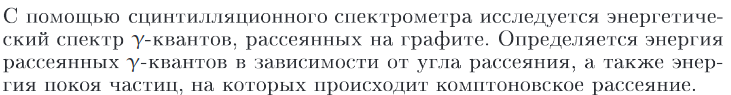
\includegraphics[width=8cm]{1.jpg}
    \caption{Схема установки}
\end{figure}
\newpage
\textbf{Применимость формулы Стокса}

Формула Стокса выводится для шара и обтекания ламинарного характера, но так как шарик круглее мы не сделаем, то определим характер обтекания:
\begin{equation}
    Re = \frac{v r \pho_l}{\eta}
\end{equation}

Обтекание является ламинарным при $Re < 0.5$

Определим также допустимое расстояние между границей жидкости и верхней меткой:

\begin{equation}
    S = v_st \tau (\frac{t}{\tau} - 1 + e^{-t/\tau})
\end{equation}
Откуда следует что $S \gg \tau v_st$ при $t \gg \tau$


\newpage
\textbf{Ход работы:}

\begin{enumerate}
    \item
    Для 4 значений температуры проведем серию из 4 бросков шариков(по 2 стальных и 2 стеклянных). Будем замерять 2 времени: между 1 и 2 отсечкой, между 1 и 3. Для рассчетов будем использовать измерения только между 1 и 3 засечкой(так как ко времени прохождения 2 засечки скорость еще может достаточно сильно увеличиваться)
    Вязкость будем определять по формуле 
    
    \begin{equation}
    \eta = \frac{2}{9} g r^2 \frac{(\rho - \rho_{l} )}{v_{st}}
    \end{equation}
    
    но если в ходе эксперимента будет обнаружена зависимость $\eta$ от радиуса шарика, то будем пользоваться более точной формулой:
    
    \begin{equation}
    \eta = \frac{2}{9} g r^2 \frac{(\rho - \rho_{l} )}{[1+2.4(r/R)]v_{st}}
    \end{equation}
    
    Также посчитаем характерное расстояние релаксации $\tau v_{opt}$.
    Далее построим график зависмости $\mathrm{ln}\eta$ от $\frac{1}{T}$ - который в теории должен быть прямой в случае ламинарного течения. По среднему коэффиценту наклона вычислим $W$.
    
    Так как часть данных в формуле для рассчета находятся из таблиц, будем считать, что такие данные вносят погрешность $\varepsilon = 0.5\%$
    
    Тогда погрешности $\eta, W$ определим из формулы для погрешности функции многих переменных:
    
    \begin{equation}
    (\frac{\sigma_\eta}{\eta})^2 = 2^2(\frac{\sigma_r}{r})^2 +  (\frac{\sigma_t}{t})^2 + 0.01
    \end{equation} 
    
    \begin{equation}
    (\frac{\sigma_W}{W})^2 = (\frac{\sigma_\eta}{\eta^2})^2 +  (\frac{\sigma_T}{T})^2
    \end{equation} 
    
    При измерениях:
    $\sigma_r = 0.025$ мм, $\sigma_T = 0.1^o$, $\sigma_t = 0.4$с (удвоенное время реакции, в которое с большой вероятностью попадут времена прохождения обоих отсечек).
    
    \item Теперь замерим $\eta$ для каждой температуры и каждого шарика.
    
    \begin{itemize}
    
    \item $T = 27.5^o C$
    
    \begin{center}
                    \begin{tabular}{|c|c|c|c|c|}
                            \hline 
                                $number$ & 1 & 2 & 9 & 10 \\
                            \hline
                                $\eta$ [мПа \cdot c]&1558&1424&1375&1429 \\
                            \hline
                                $\sigma_\eta$ [мПа \cdot c]&88&77& 54&56 \\
                            \hline
                                $\varepsilon_\eta$[\%] &6&5&4&4 \\
                            \hline
                                $Re$ &0.0&0.1&0.2& 0.2 \\
                            \hline
                                 $\tau v_{opt}$ [см] &0.02&0.08&0.15&0.16&
                            \hline
                    \end{tabular}
        \end{center}
        
    \item $T=36.5^o C$
     \begin{tabular}{|c|c|c|c|c|}
                            \hline 
                                $number$ & 3 & 4 & 11 & 12 \\
                            \hline
                                $\eta$ [мПа \cdot c]&862&865&776& 868 \\
                            \hline
                                $\sigma_\eta$ [мПа \cdot c]&53&55& 39&45 \\
                            \hline
                                $\varepsilon_\eta$[\%] &6&6&5&5 \\
                            \hline
                                $Re$ &0.1&0.1&0.5&0.5 \\
                            \hline
                                                             $\tau v_{opt}$ [см] &0.11&0.17&  0.4&  0.5&
                            \hline
                    \end{tabular}
                    
    \item $T=47.1^o C$
     \begin{tabular}{|c|c|c|c|c|}
                            \hline 
                                $number$ & 5 & 6 & 13 & 14 \\
                            \hline
                                $\eta$ [мПа \cdot c]&475&443&481& 484 \\
                            \hline
                                $\sigma_\eta$ [мПа \cdot c]&36&37&35&36 \\
                            \hline
                                $\varepsilon_\eta$[\%]&8&8&7&8 \\
                            \hline
                                $Re$ &0.3&0.5&1.5&1.5 \\
                            \hline
                                                            $\tau v_{opt}$ [см] &0.3&0.5&1.4&  1.5&
                            \hline
                    \end{tabular}
    \item $T=54.9^o C$
     \begin{tabular}{|c|c|c|c|c|}
                            \hline 
                                $number$ & 7 & 8 & 15 & 16 \\
                            \hline
                                $\eta$ [мПа \cdot c]&293&295&273&293\\
                            \hline
                                $\sigma_\eta$ [мПа \cdot c]&25&34& 29&30 \\
                            \hline
                                $\varepsilon_\eta$[\%] &9&12&11&10
                                \\
                            \hline
                                $Re$ &0.5&1.5&3.9&3.7 \\
                            \hline
                                                              $\tau v_{opt}$ [см] & 0.4&1.9&3.6&3.4&
                            \hline
                    \end{tabular}
                    
            \end{itemize}
    \item
     Заметно, что для больших шаров и температур применимость модели должна уменьшеаться из-за большого числа Рейнольдса.
    
       В целом видно, что $\eta$ не зависит от радиуса, но заметны систематические ошибки в некоторых случаях.
       Такие эксперименты стоит отбросить.
       По оставшимся вычислим среднее $\eta(t)$
     
     \begin{tabular}{|c|c|c|c|c|}
                            \hline 
                                $T[^o C]$ &27.5&36.5&47.1&54.9 \\
                            \hline
                                $\eta(t)$ [мПа \cdot c]&1427&    864&479&293\\
                            \hline
                                $\sigma_\eta$ [мПа \cdot c] &67&51&35& 30 \\
                            \hline
                                $\varepsilon_\eta$[\%] &5&6&8&10 \\
                            \hline
                    \end{tabular}

    Построим график $\mathrm{ln} \eta$ от $\frac{1}{T}$:
    

    Тогда получим значение для энергии активации: 
    
    $W = (8.00 \pm 0.25) \cdot 10^{-20}$ Дж и $\varepsilon_W \sim 3\%$
    
    \begin{figure}[htp]
    \centering
    \includegraphics[width=10cm]{graph.png}
    \caption{}
\end{figure}

    \begin{figure}[htp]
    \centering
    \includegraphics[width=10cm]{data.png}
    \caption{}
\end{figure}

\end{enumerate}
\end{document}